\documentclass{article}
\usepackage{tikz}

\begin{document}
\section*{Multi-Figure Basic Fixture}
This file has multiple TikZ figures and ordinary text in between them.
It intentionally avoids custom macros, tikzset/tikzstyle commands, and custom color definitions.

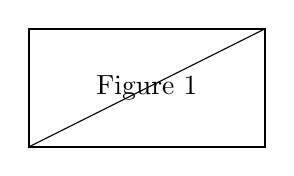
\begin{tikzpicture}
  \draw[thick] (0,0) rectangle (3,1.5);
  \draw (0,0) -- (3,1.5);
  \node at (1.5,0.75) {Figure 1};
\end{tikzpicture}

Some regular paragraph text between figure 1 and figure 2.

\begin{tikzpicture}
  \draw[->] (0,0) -- (3,0) node[right] {$x$};
  \draw[->] (0,0) -- (0,2.2) node[above] {$y$};
  \draw[dashed] (0.5,0.5) -- (2.4,1.8);
\end{tikzpicture}

More text between figure 2 and figure 3, including inline math: $a^2+b^2=c^2$.

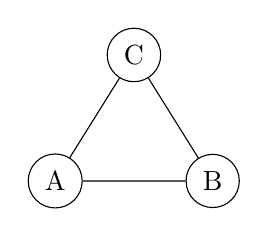
\begin{tikzpicture}
  \node[draw, circle] (A) at (0,0) {A};
  \node[draw, circle] (B) at (2,0) {B};
  \node[draw, circle] (C) at (1,1.6) {C};
  \draw (A) -- (B) -- (C) -- (A);
\end{tikzpicture}

Final paragraph before the last figure.

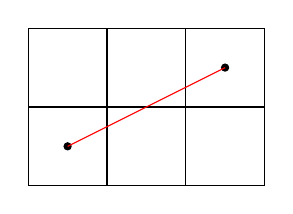
\begin{tikzpicture}
  \draw (0,0) grid (3,2);
  \fill (0.5,0.5) circle (1.5pt);
  \fill (2.5,1.5) circle (1.5pt);
  \draw[red] (0.5,0.5) -- (2.5,1.5);
\end{tikzpicture}

\end{document}
